\documentclass[usenatbib]{mnras}
\usepackage[T1]{fontenc}
\usepackage{ae,aecompl}

\usepackage{graphicx}	% Including figure files
\usepackage{amsmath}	% Advanced maths commands
\usepackage{amssymb}	% Extra maths symbols
\usepackage{subfig}
\usepackage{array}

\usepackage{multirow}
\usepackage{multicol}
\usepackage{blindtext}
\newcolumntype{?}{!{\vrule width 1pt}}
\newcommand{\Msun}{\,{\rm Mpc}$_{\odot}$\,}
\newcommand{\Mpch}{\,{\rm Mpc}\,\ifmmode h^{-1}\else $h^{-1}$\fi}
\newcommand{\kpch}{\,{\rm kpc}\,\ifmmode h^{-1}\else $h^{-1}$\fi}
\newcommand{\kpc}{\,{\rm kpc}\,}


\title[Dark matter halo shapes at $z=0$] {Dark matter halo shapes at
  $z=0$ in the Auriga simulations} 
\author[Jesus Prada,  Jaime E. Forero-Romero, Volker Springel ]{
Jesus Prada,$^{1}$\thanks{E-mail: jd.prada1760@uniandes.edu.co}
Jaime E. Forero-Romero,$^{1}$
Volker Springel$^{2}$
\\
% List of institutions
$^{1}$Departamento de F\'isica, Universidad de los Andes, Cra. 1 No.
18A-10, Edificio Ip, Bogot\'a, Colombia\\
$^{2}$Max-Planck-Institut f\"ur Astrophysik, Karl-Schwarzschild-Str. 1, D-85741 Garching, Germany\\
}

% These dates will be filled out by the publisher
\date{Accepted XXX. Received YYY; in original form ZZZ}

% Enter the current year, for the copyright statements etc.
\pubyear{2019}

% Don't change these lines
\begin{document}
\label{firstpage}
\pagerange{\pageref{firstpage}--\pageref{lastpage}}
\maketitle

% Abstract of the paper
\begin{abstract}
We present shape measurements of Milky Way sized dark matter halos at
redshift $z=0$ in a suite of 30 zoom simulations from the Auriga
project. 
We compare the results in full magnetohydrodynamics against dark
matter only physics. 
We find a strong influence of baryons in making dark matter halos
rounder at all radii compared to its dark matter only counterparts.
At distances $\lesssim 30$ kpc, rounder dark matter distributions
correlate with extended massive stellar discs and low gas 
densities.  
We measure the alignment between the halo and the stellar disc and
find almost perfect alignment at $0.25R_{200}\sim56$ kpc.   
In some cases the alignment between the two components significantly
changes as a function of radius implying that the halo shape twists;
this effect correlates with extended stellar discs and
low gas densities and is almost absent in the dark matter only
simulations.  
In a comparison against observational constraints  we find that $20\%$
of halos are consistent with observational results derived
from the Pal 5 stream that favor an almost spherical shape.
Including baryons is a required element to achieve this
level of agreement. In contrast, none of the simulations (dark matter
only nor with baryons) match the constrains derived from the
Sagittarius stream favoring an oblate dark matter halo.
\end{abstract}

% Select between one and six entries from the list of approved keywords.
% Don't make up new ones.
\begin{keywords}
galaxies: evolution --- galaxies: formation --- galaxies: haloes ---
dark matter
\end{keywords}

%%%%%%%%%%%%%%%%%%%%%%%%%%%%%%%%%%%%%%%%%%%%%%%%%%

%%%%%%%%%%%%%%%%% BODY OF PAPER %%%%%%%%%%%%%%%%%%

\section{Introduction}

Our physical picture of the Universe as a whole has be shaped by
accurate observations and modeling of our own Galaxy. 
Explaining the matter budget and kinematical state of the Milky Way
(MW) is  equivalent to figuring out its formation process in a
cosmological context. 
As a first approximation, the MW morphology and
separation into global kinematically coherent components, such as its
disc and bulge, can be used to support the  existence of a Dark Matter
(DM) component to explain its dynamics around the solar neighborhood
\citep{2000MNRAS.311..361O,2009PASJ...61..227S,2010JCAP...08..004C,2013ApJ...779..115B,Iocco15}. 


A more detailed description of the full three-dimensional MW
gravitational potential is possible through the interpretation of 
fossil records of stellar streams.
These remanents, resulting from infalling globular clusters or
satellite galaxies that got tidaly disrutpted by the gravitational
potential of the Milky Way, allow in principle tighter constrains 
on the shape of the dark matter halo in outter regions of our Galaxy
\citep{1998ApJ...495..297J,1999MNRAS.307..495H, 1999MNRAS.307..877T}
than dynamical measurements close to the solar neighborhodd.

The observational constraints on the gravitational potential shape can then
be confronted against the expectations from different galaxy formation
models in an explicit cosmological context.
For instance, in the current dominant paradigm of Cold Dark Matter
(CDM) dominated Universe galaxies are expected to be hosted by
triaxial DM halos. To what extent the CDM expectations are born out by
observations in our Galaxy? Can the MW's DM halo shape be considered
typical or atypical in a cosmological context?


These two questions have been difficult to address because for a long
time it was difficult to produce realistic galactic discs within the
CDM context.
The success of such enterprise has been the result of high numerical
resolution and the understanding that baryonic effects such as stellar
feedback and black hole feedback play an important role in forming a
galactic disc resembling the Milky Way.
Along the way numerical experiments show that the baryonic effects also impact
the dark matter halo shape making the halo rounder than it otherwise
be in a dark matter only simulation
\citep{Dubinski94,Debattista08,Kazantzidis10,Abadi10,Bryan13,Chua19,Artale19}. 
High resolution simulations have also allowed detailed studies of the
alignment between the stellar disc and the dark matter halo
\citep{Bailin05,DeBuhr12,Debattista13,Gomez17}.





Observational constraints of the dark matter halo have been in
tension during the last decade. 
One can find studies favoring prolate
\citep{Banerjee_and_Chanda_2011,Bowden_et_al._2016},  oblate
\citep{LM10,Deg_and_Widrow_2013,Vera-Ciro_and_Helmi_2013} and
spherical configurations \citep{Bovy16}.  
Constraints from modeling of stellar streams discard the prolate
configuration \citep{LM10,Pearson_et_al._2015,Bovy16} although some other studies
still doubt that stellar streams can be used to constrain the halo
shape once other assumptions, such as the density profile, are relaxed
\citep{Ibata_et_al._2013}. 



In this paper we contribute to the debate by reporting measurements of
the DM halo shape in MW type galaxies from state-of-the-art simulations from the
Auriga project.
These simulations have large enough numerical resolution, and explicit
cosmological context and an appropriate feedback physics to produce
realistic MW discs.
This paper is structured as follows. 
In Section \ref{sec:numerical} we present the most relevant details of
the simulations, in Section \ref{sec:method} we present the method
that we use to measure the DM halo shape. 
In Section \ref{sec:results} we present our results focusing on the
radial shape trends at $z=0$ and the alignments with the stellar disc.
We discuss our results in Section \ref{sec:discussion} to place them
into the context of other numerical work, explore correlations of the
shape with baryonic properties in the disc and finally make a direct
comparison against observational constraints for the MW's dark matter halo shape.
We finalize with our conclusions in Section \ref{sec:conclusions}.


\section{Numerical Simulations}
\label{sec:numerical}

The Auriga project offers cosmological zoom in simulations of MW-sized 
dark matter halos in a $\Lambda$CDM cosmology. 
This simulations come in two versions: dark matter only (DMO) and
baryonic physics including magetohydrodynamics (MHD).
A detailed description of the simulations and their disc properties
can be founc in \citep{auriga}, here we summarize its main features.

The objects in the simulations were selected from a set of 30
isolated halos in the Evolution and Assembly of GaLaxies and their
Environments (EAGLE)  project \citep{Eagle}.   
These halos were randomly selected from a sample of the most isolated
halos at $z=0$ whose virial mass $M_{200}$ was between $10^{12}M_\odot$ and
$2\times 10^{12}M_\odot$. 
The cosmological parameters in these simulatins correspond to
$\Omega_m=0.307$, $\Omega_b=0.048$, $\Omega_\Lambda=0.693$ and a
dimensionless Hubble parameter $h=0.6777$ \citep{2014A&A...571A..16P}

The selected halos were re-simulated at higher resultion by applying a
zoom-in technique with varying physical realism using the moving-mesh AREPO code
that includes gravity, ideal magnetohydrodynamics,  phenomenological
descriptions for star formation, chemical enrichment from supernovae
and its stellar feedback.   
The simulation also follows the formation and evolution of black holes
together with the Active Galactic Nuclei feedback
\citep{arepo,2013MNRAS.432..176P}. 




The 30 zoom-in halos have a dark matter particle mass of $\sim 3\times
10^5$\Msun while the barynic mass resolution is $\sim 5\times 10^4$\Msun.
The softening lenght for gravitational force computation for stellar
particles and high-resolution dark matter particles 
is fixed to be 500 $h^{-1}$ pc in comoving coordinates up to $z=1$,
and 396 pc in physical coordinates afterwards.
The gravitational softening lenght for gas cells changes with the mean
cell radius but is limited to be larger than the stellar softening
lenght and 1850 pc physical. 
From now on we refer to the haloes simulated with baryonic physics as the
MHD sample and to the haloes simulated with dark matter only as the
DMO sample.


\begin{figure*}
  \centering
  \subfloat[DMO simulation. Shape at small
    radius.]{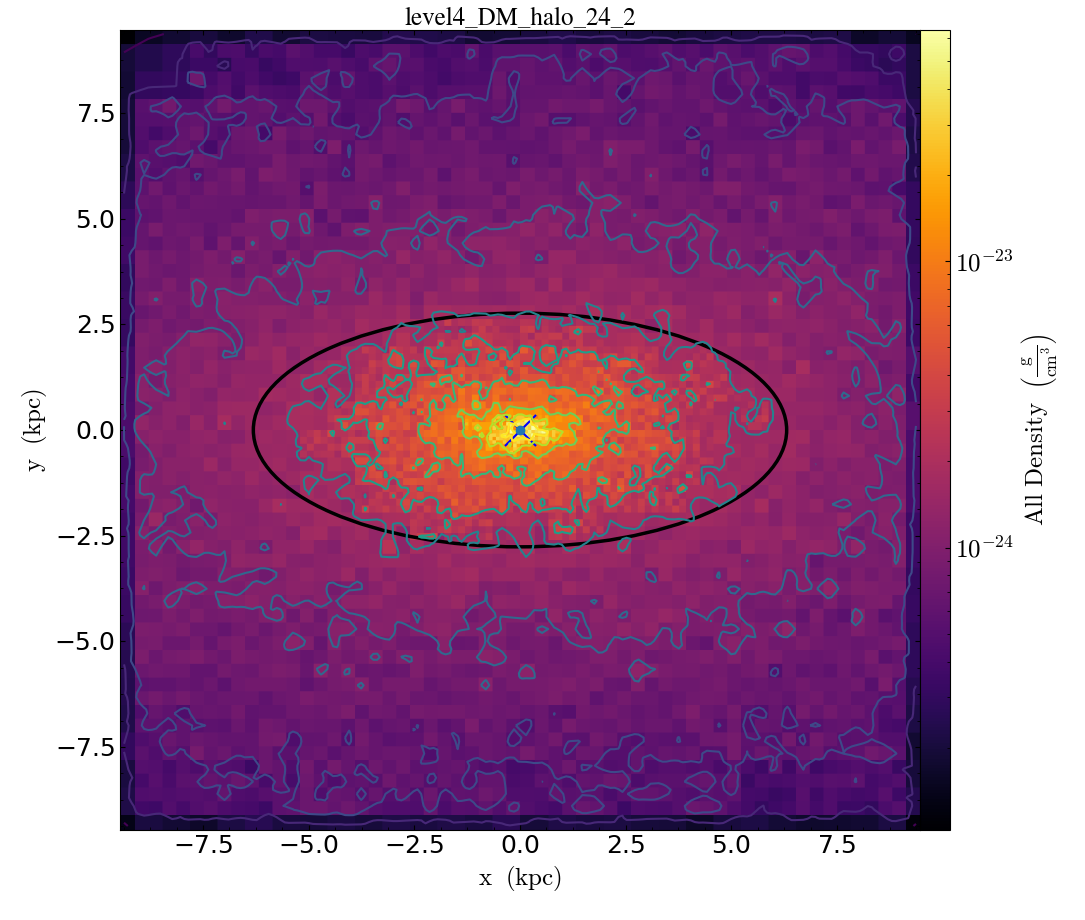
\includegraphics[width=0.5\textwidth]{level4_DM_halo_24_2.png}}  
  \hfill
  \subfloat[DMO simulation. Shape at large
    radius.]{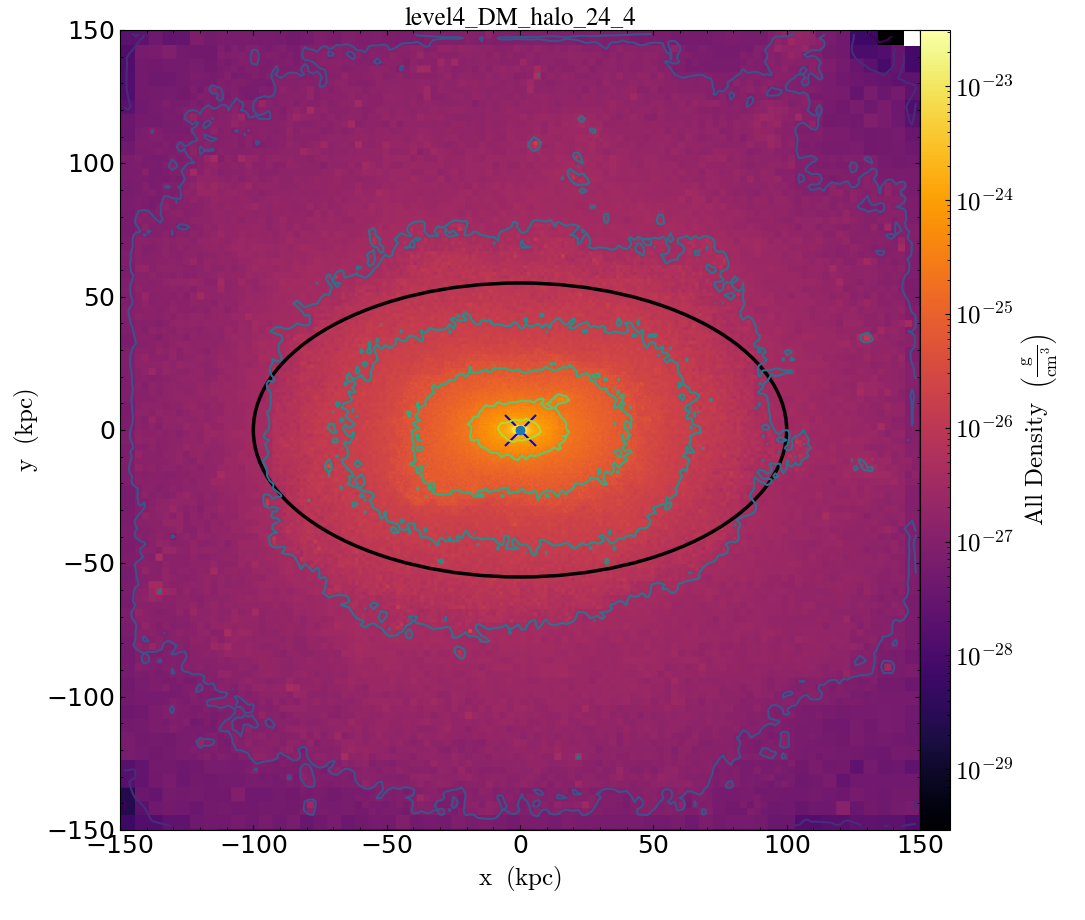
\includegraphics[width=0.5\textwidth]{level4_DM_halo_24_4.png}}  
  \hfill 

  \subfloat[MHD simulation. Shape at small
    radius.]{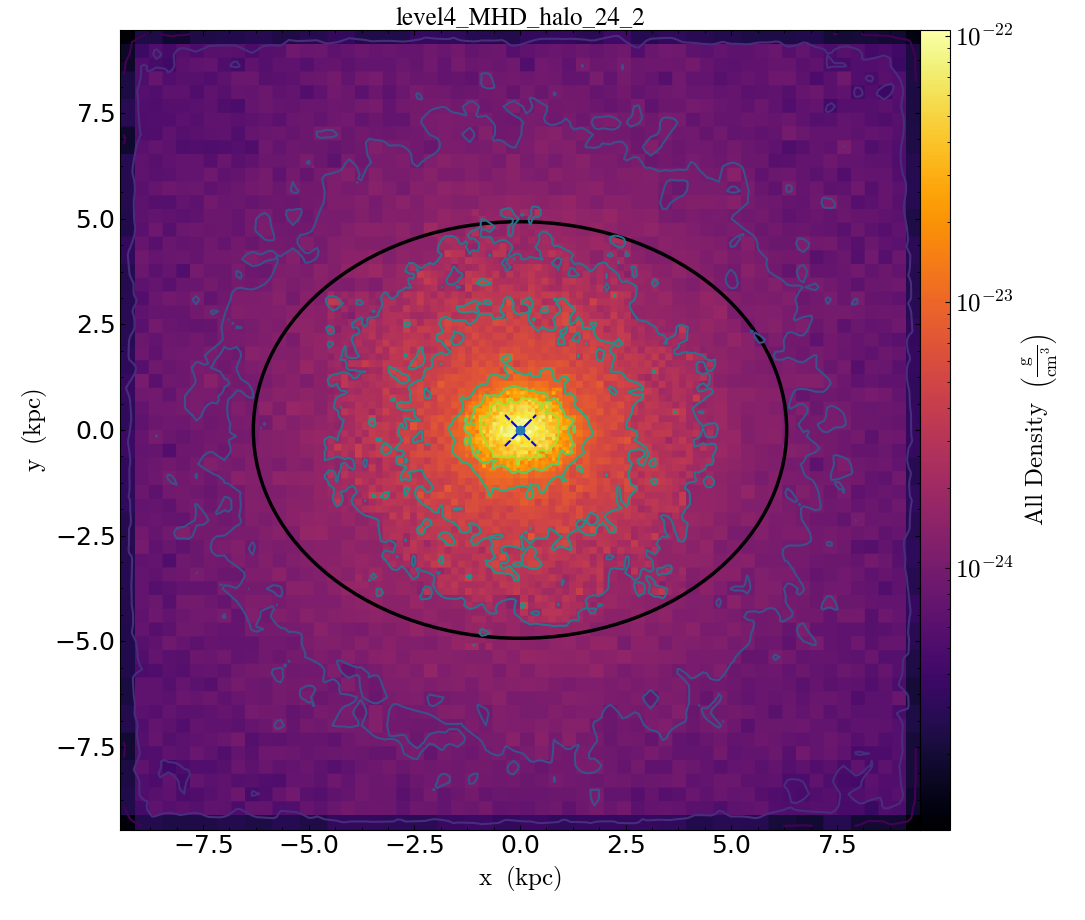
\includegraphics[width=0.5\textwidth]{level4_MHD_halo_24_2.png}}  
  \hfill
  \subfloat[MHD simulation. Shape at large
    radius.]{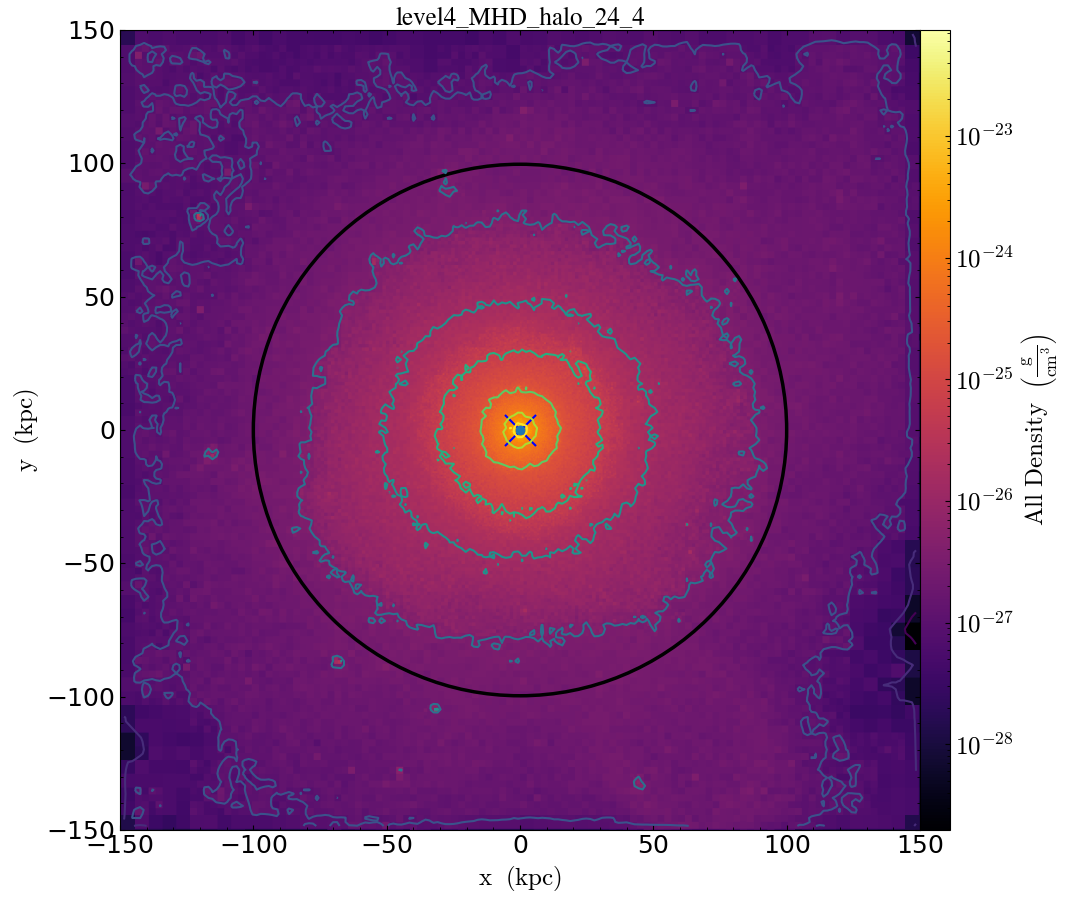
\includegraphics[width=0.5\textwidth]{level4_MHD_halo_24_4.png}}  
  \hfill 
  \caption{DM density in logarithmic scale within a slice of one tenth
    of the virial radius in width. 
    The cut is perpendicular to the short axis of the inertia tensor ellipsoid.
    The black ellipses show the results of the fitting procedure. 
    Upper panels correspond to DMO simulations, lower panels to MHD
    simulations.
    All cases correspond to \texttt{Level4} resolution.
    Left panels show data at small radii, while right panels at large
    radii.    
    This halo showcases the most noticeable effect in all halos
    across the Auriga simulations: DM halos are rounder at all radii
    after baryonic physics is included.}
\label{fig:slices}
\end{figure*}


 
\begin{figure*}
\begin{center}
\subfloat[DMO simulations.]{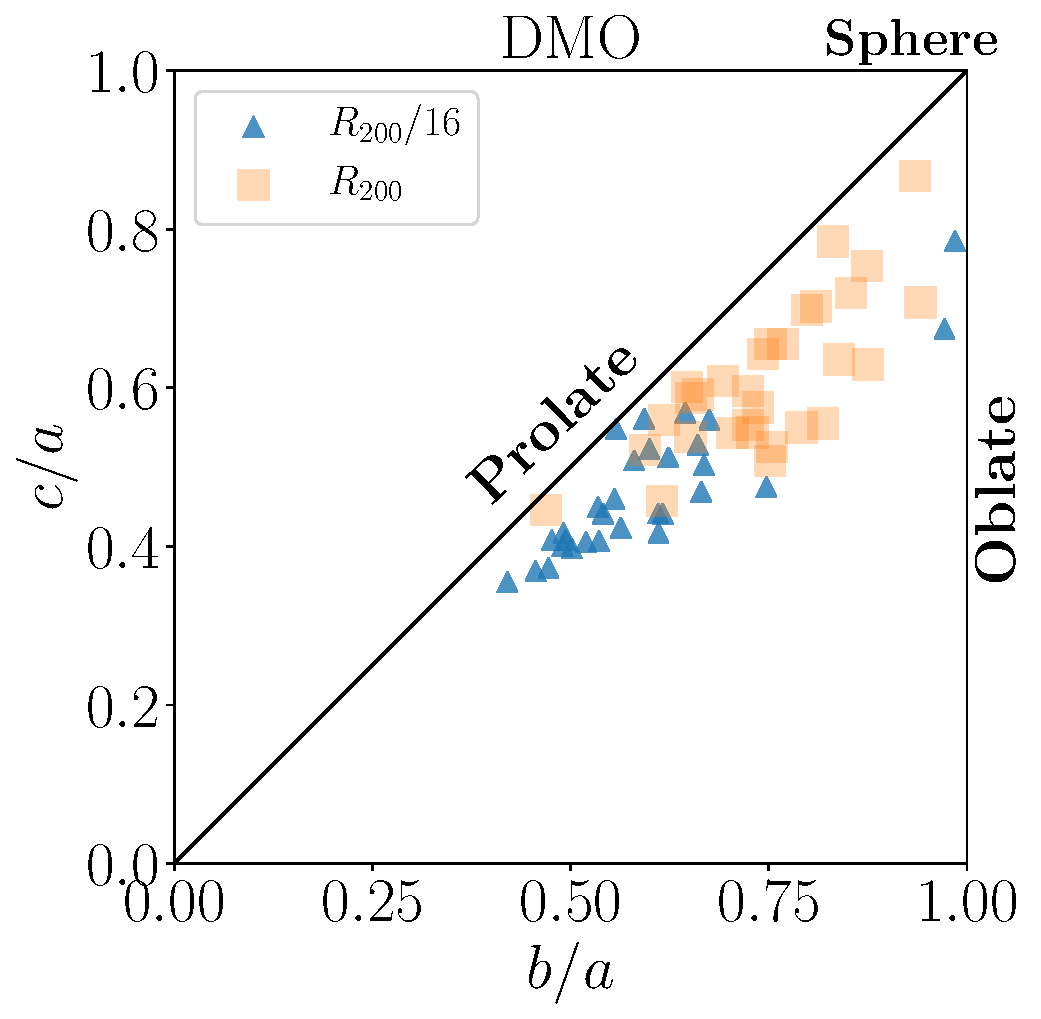
\includegraphics[width=0.8\columnwidth]{Lvl_4_Triax_Plane_DM.pdf}}
\subfloat[MHD simulations.]{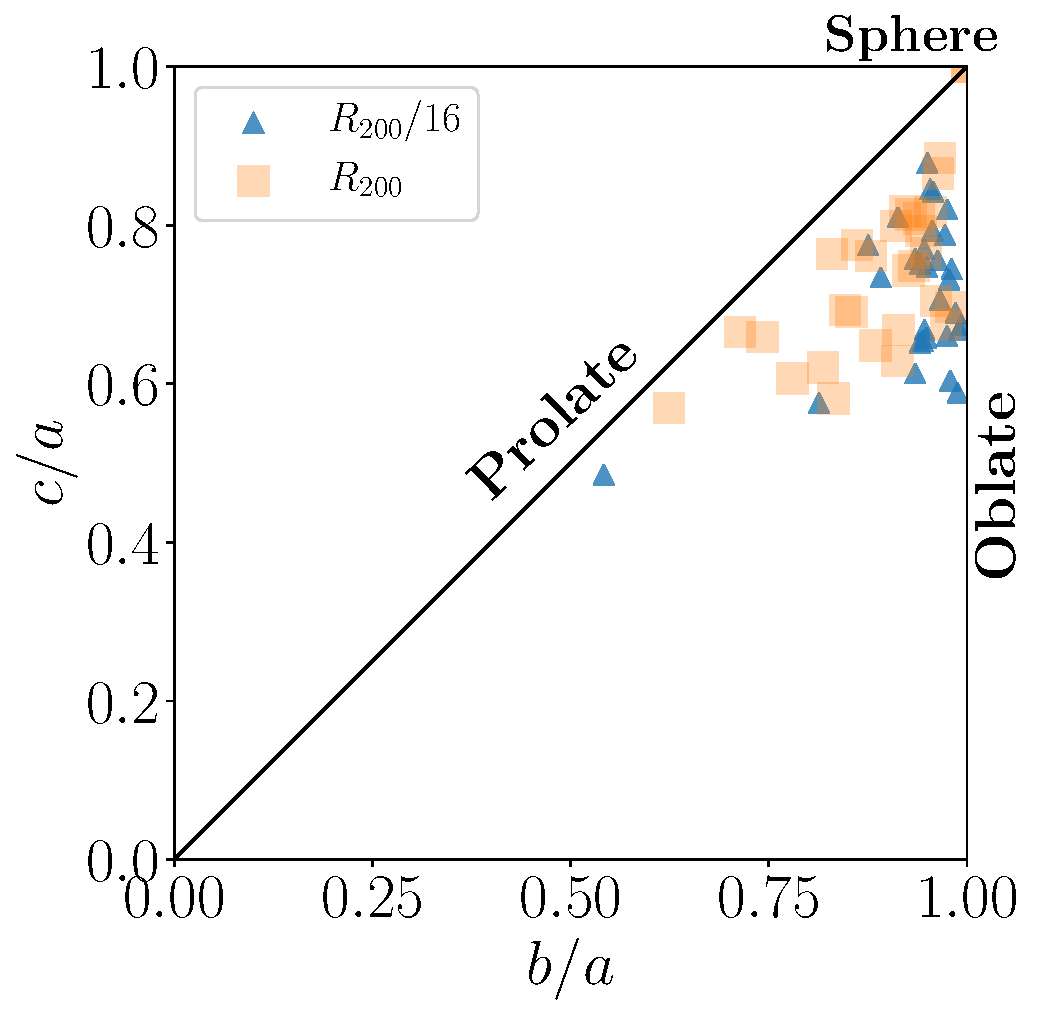
\includegraphics[width=0.8\columnwidth]{Lvl_4_Triax_Plane_MHD.pdf}}
\end{center}
\caption{Axial ratios for all halos in the simulation.
  Left/right panels correspond to DMO/MHD simulations, respectively.
  Triangles (squares) represent the measurements at $R_{200}/16$
  ($R_{200}$) which correspond to physical distances of $14\pm 1$ kpc
  ($230\pm 15$ kpc) respectively.
  Here we can visualize three main trends for the whole halo population.
  First, in DMO simulations halos are rounder in the outskirts
  than in the inner part.
  Second, halos in MHD are rounder than its DMO counterparts.
  Third, halos in MHD are less triaxial in the inner regions than in
  the outskirts.}
  \label{fig:triaxiality_plane}
\end{figure*}


\begin{figure*}
\subfloat[DMO simulations.]{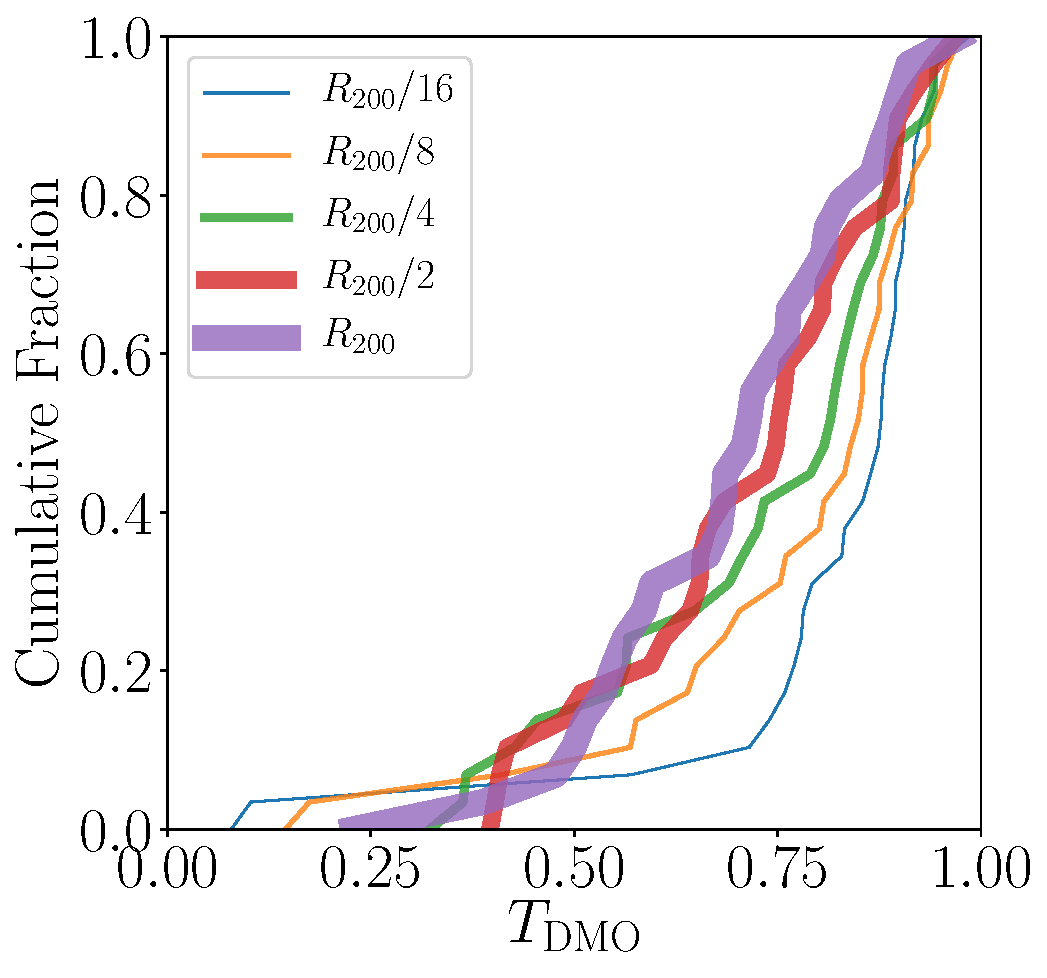
\includegraphics[width=0.8\columnwidth]{triaxialiy_distro_DM.pdf}}
\subfloat[MHD simulations.]{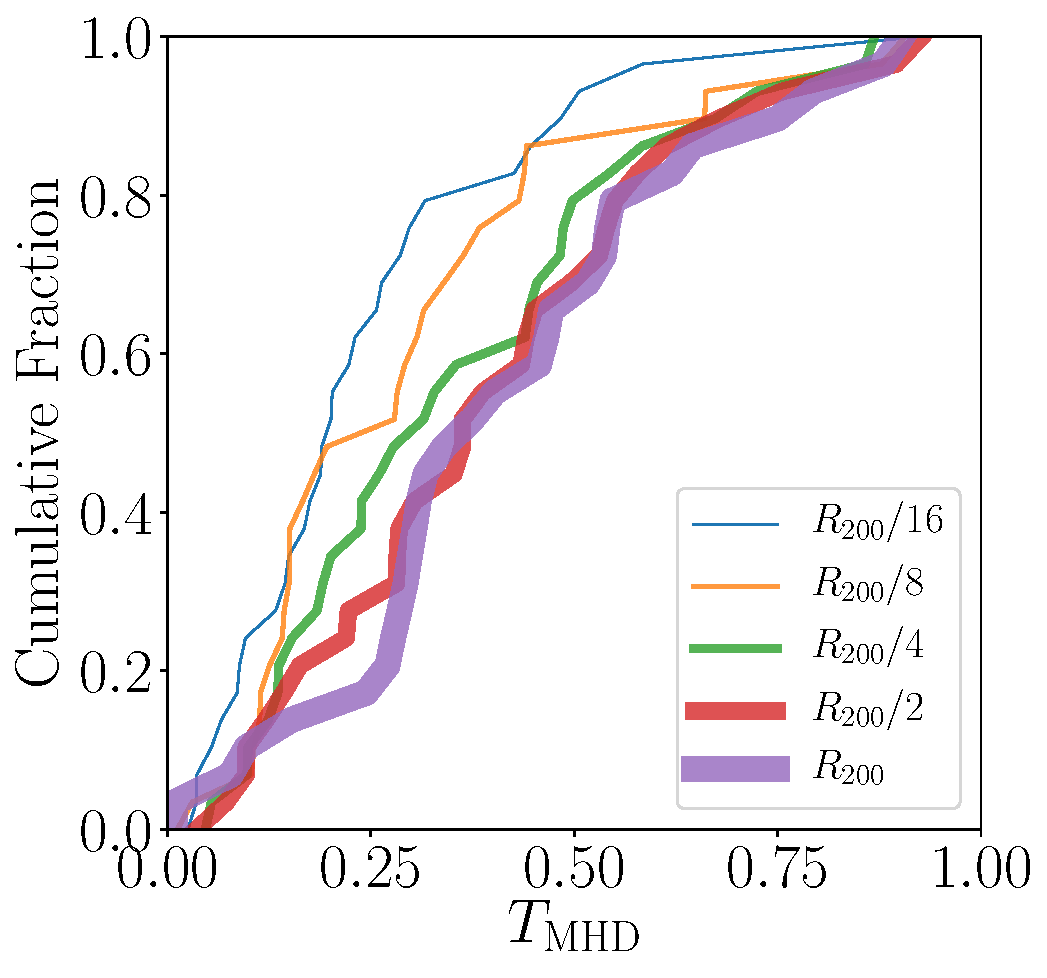
\includegraphics[width=0.8\columnwidth]{triaxialiy_distro_MHD.pdf}}
\caption{Cumulative distribution for the triaxiality at five different radii.
  Right/left panel correspond to DMO/MHD simulations, respectively. 
  In DMO simulations the median triaxiality at all radii is larger
  than $0.5$; only for $20\%$ the triaxility is smaller than $0.5$.
  Furthermore, the triaxility increases as one moves towards the inner
  part of the halo.
  In MHD simulations the situation is reversed.
  The median triaxility at all radii is smaller than $0.5$.
  Moving towards the stellar disc the triaxility decreases towards a median
  value of $T=0.15$.}
\label{fig:triaxial_cumulative}
\end{figure*}


\begin{figure}
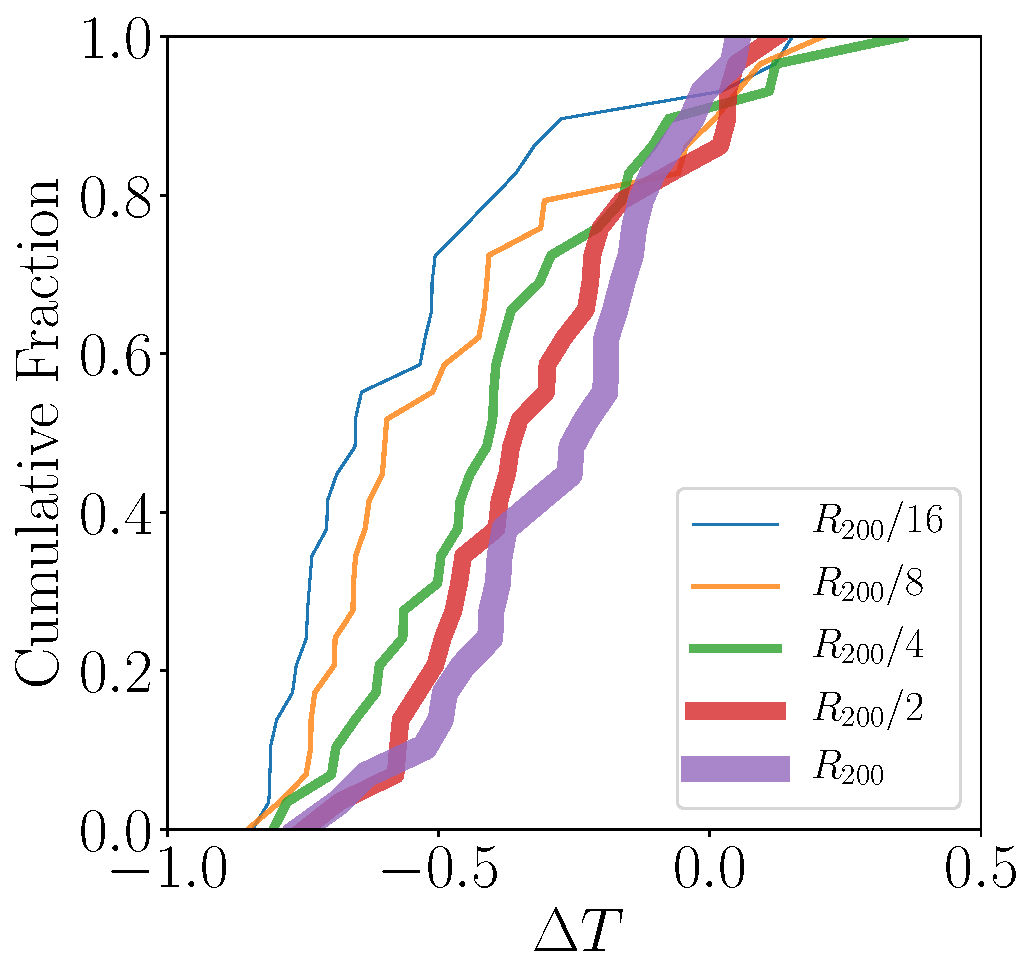
\includegraphics[width=0.9\columnwidth]{delta_triaxiality_distro.pdf}
\caption{
  Cumulative distribution for the change in triaxility $\Delta T=T_{\rm
    MHD}-T_{\rm DMO}$ for the same radii used in Figure
  \ref{fig:triaxial_cumulative}. 
  At the virial radius all the halos become less triaxial in the MHD
  simulations. 
  The change in triaxility becomes stronger in the inner regions of
  the dark matter halo.}
\label{fig:delta_triaxial_cumulative}
\end{figure}



\begin{figure*}
\begin{center}
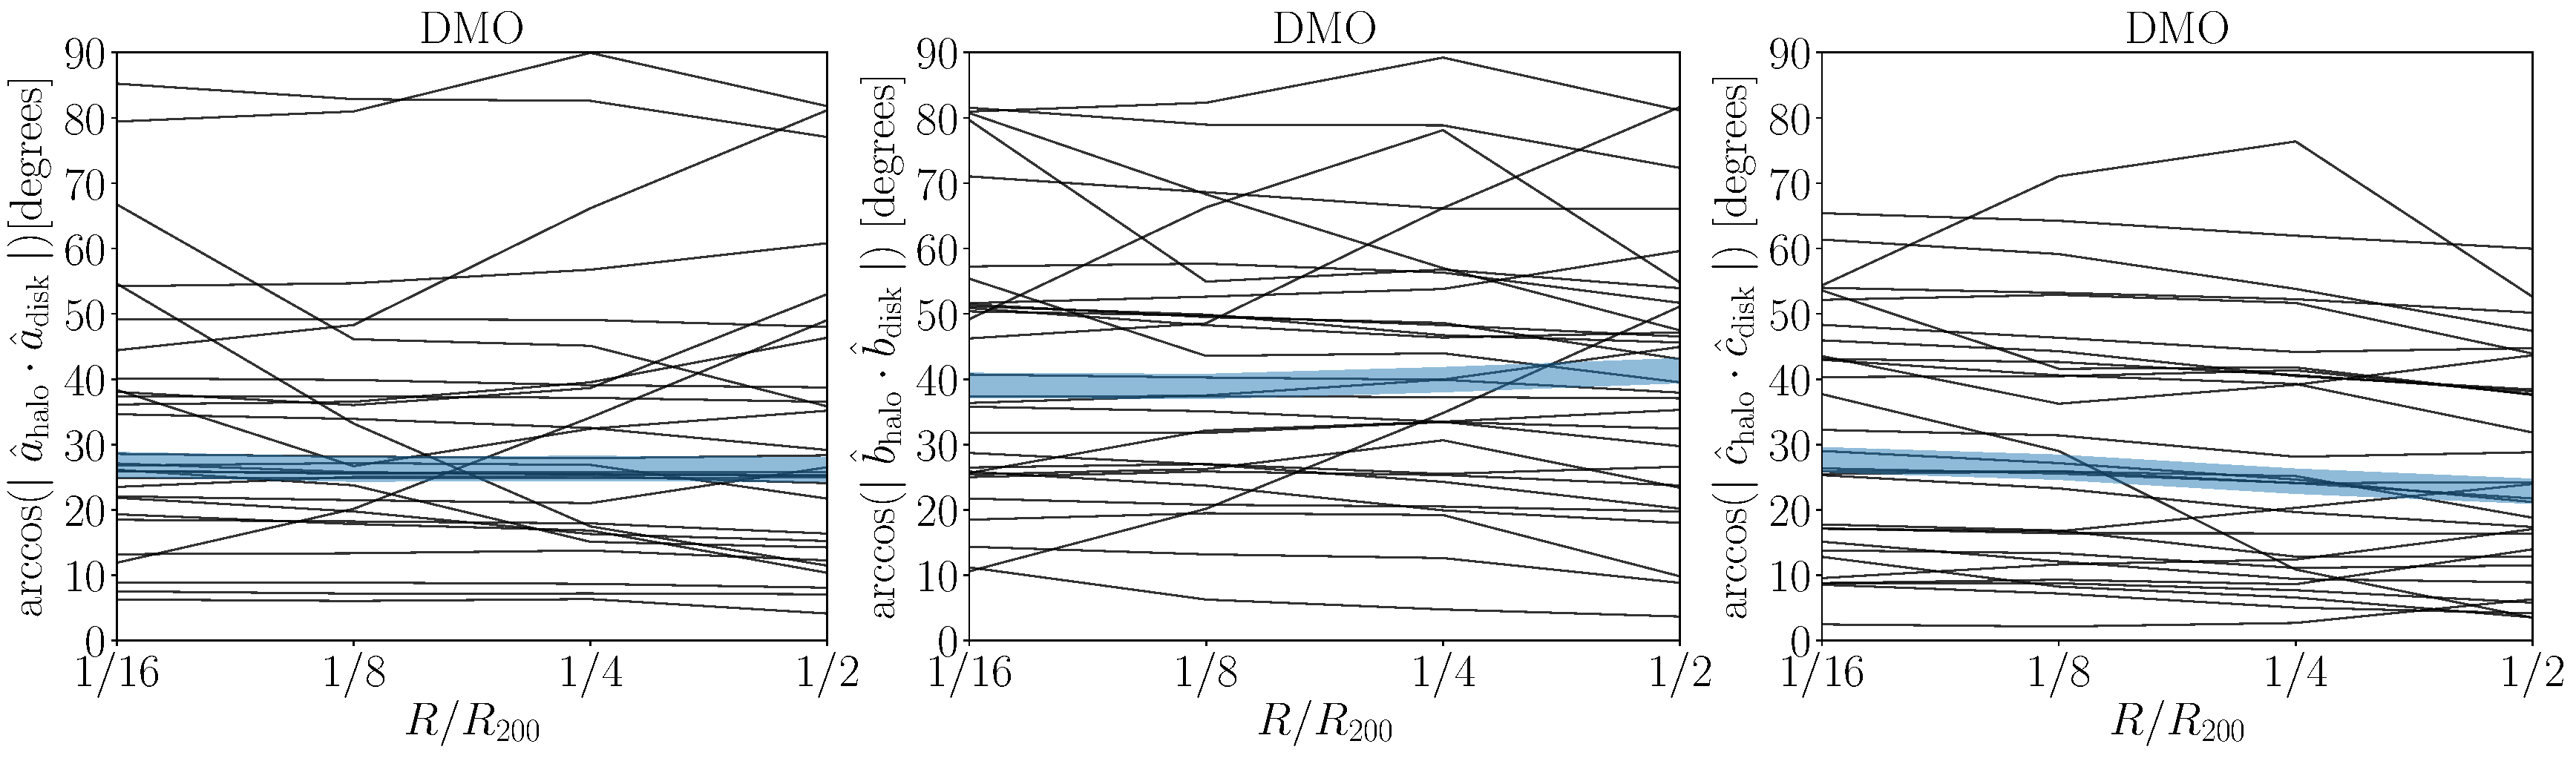
\includegraphics[width=1.0\textwidth]{angles_alignment_DM.pdf}
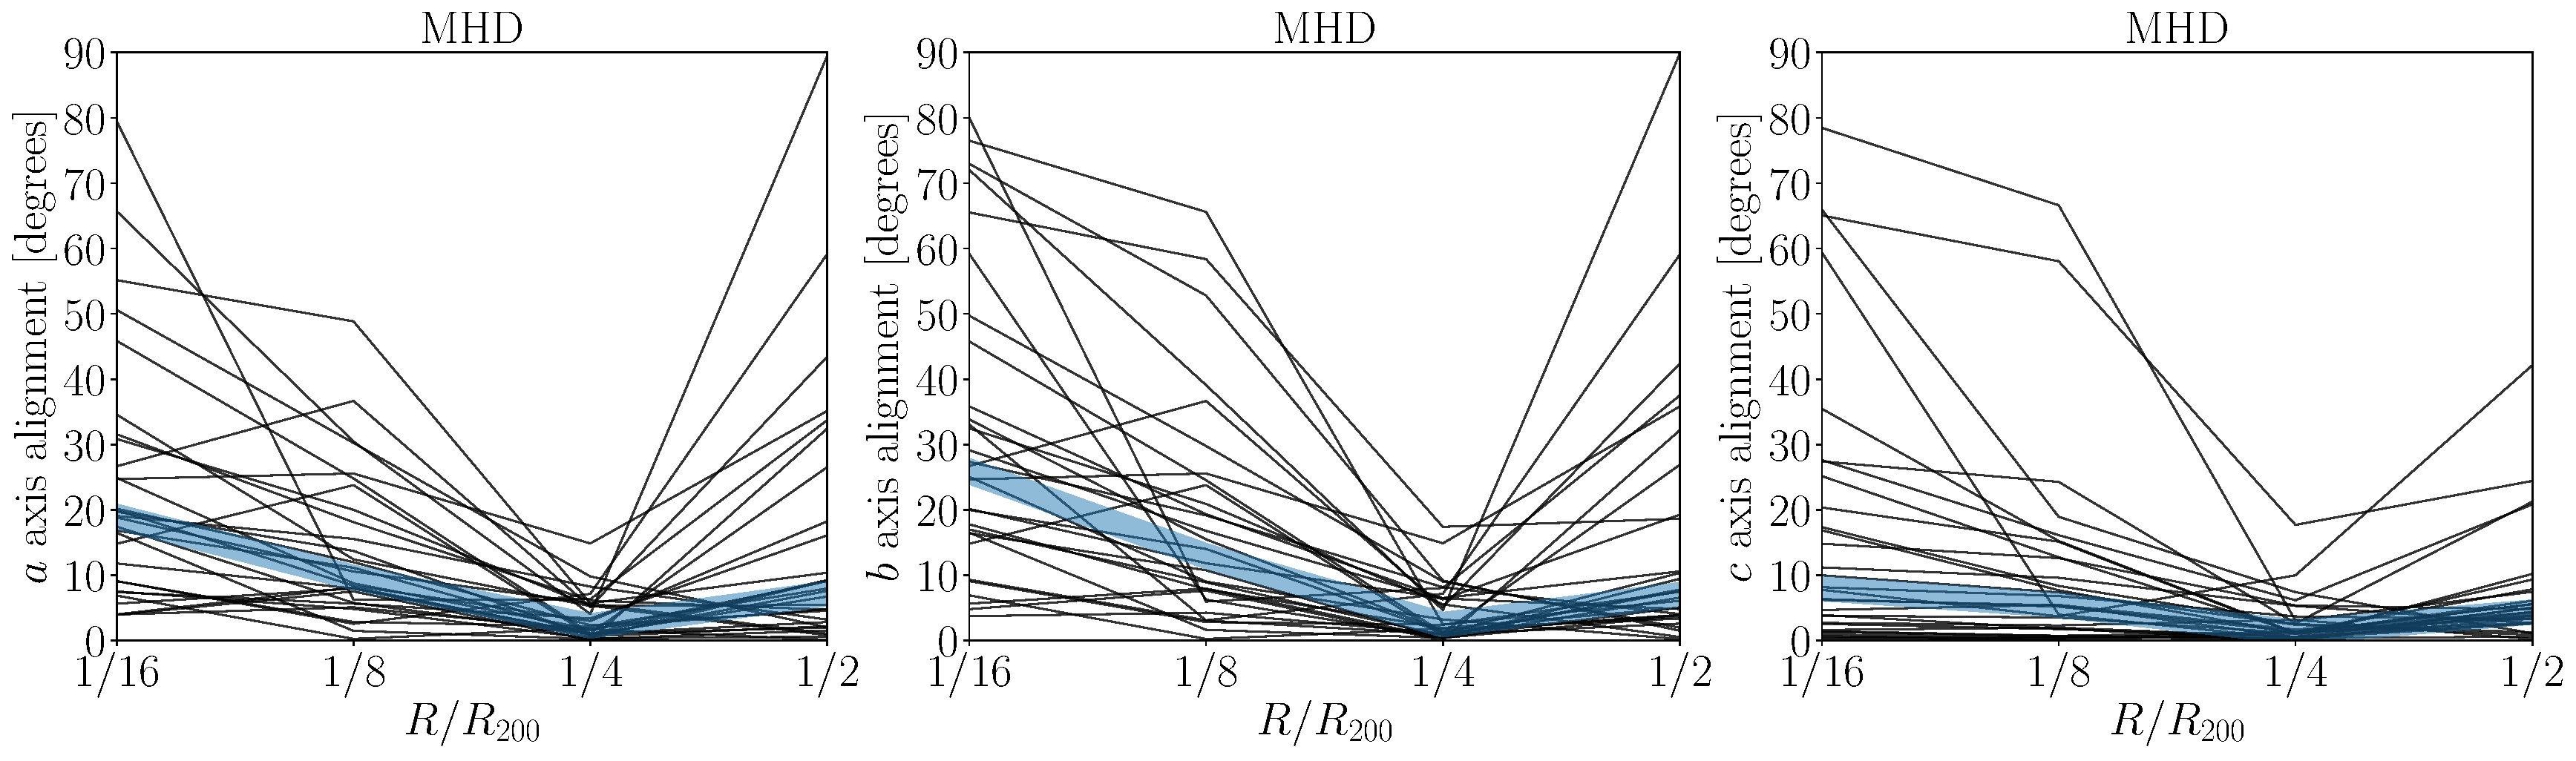
\includegraphics[width=1.0\textwidth]{angles_alignment_MHD.pdf}
\end{center}
\caption{Angles between the
  principal axis of the halo shape and the principal axis of the
  stellar disc in the MHD simulations at four different radii $\leq 0.5R_{200}$.
  Thin lines correspond to each one of the thirty halos in our sample,
  while the thick line traces the median value.
  Each panel compares the alignment of the corresponding
  major/middle/minor axis both in the halo and the stellar disc.
  In the upper row the haloes come from the DMO simulation, 
  showing that the ellipsoids describing the
  shape are constant as a function of radius for the most part of the
  sample.
  In the lower row the haloes come from the MHD simulation providing a 
  self-consistent comparison with the stellar discs. 
  In this case the dark matter shells twist in all the halos.
  The degree of this twisting is different in each halo.
  Interestingly, an almost perfect halo-disc alignment happens across
  the sample at an intermediate radius of $0.25R_{200}$ ($56\pm 4$kpc).
}
\label{fig:cumulative_alignment}
\end{figure*}


\begin{figure*}
\begin{center}
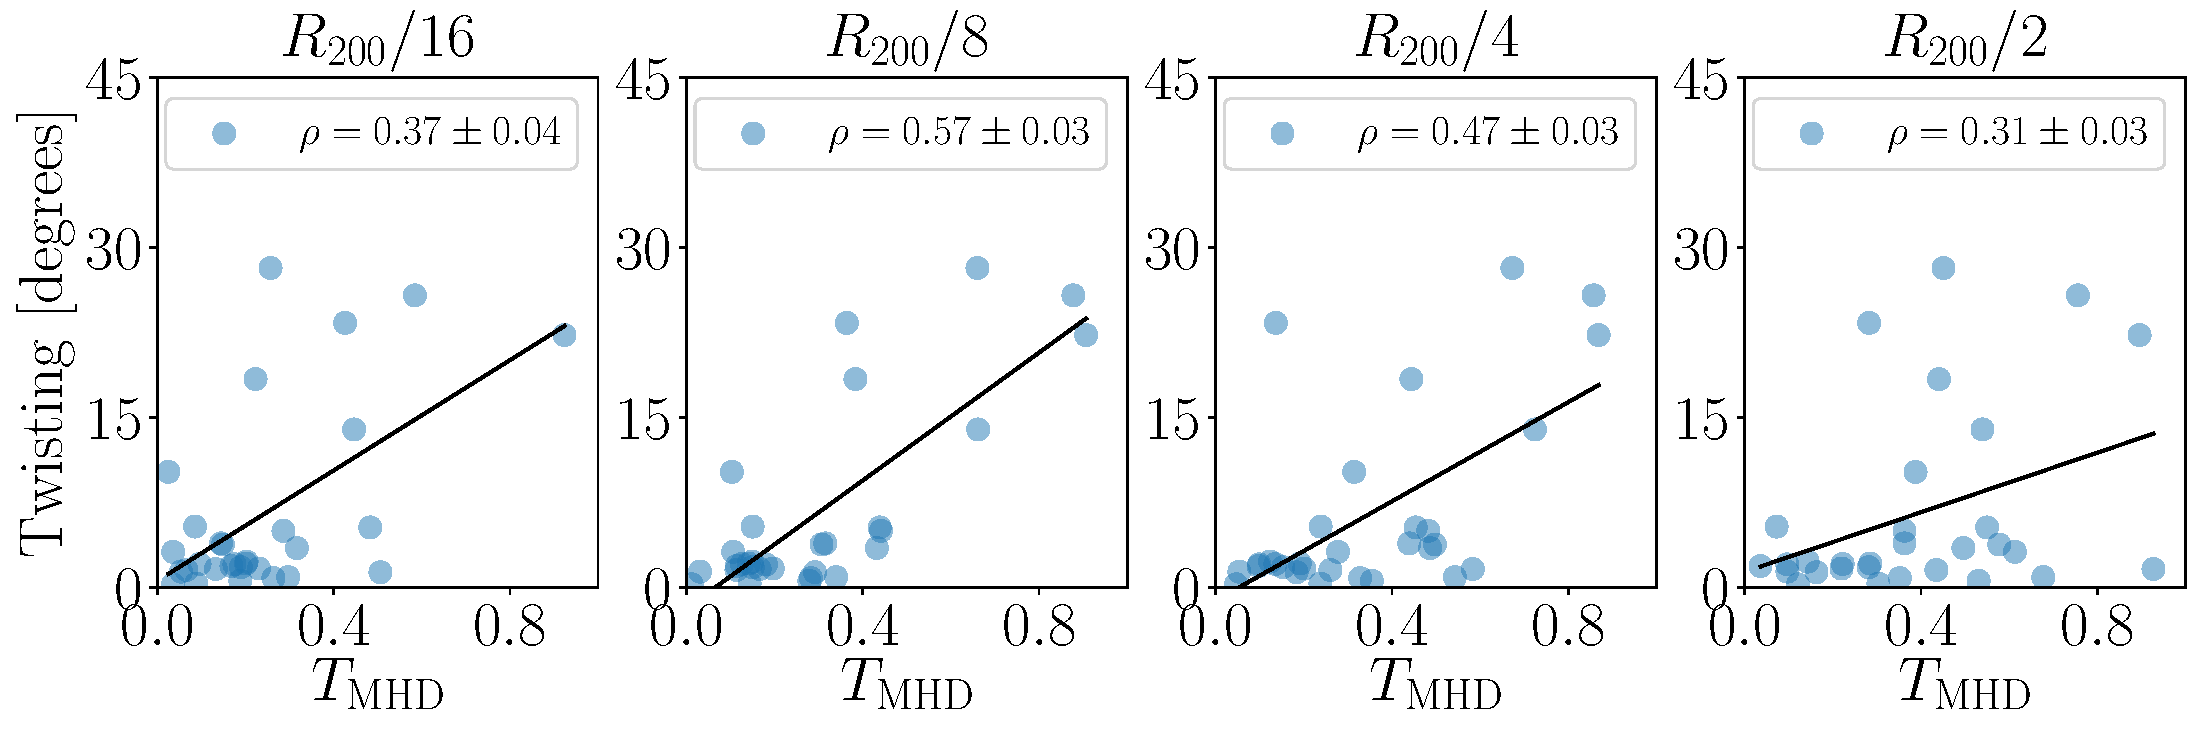
\includegraphics[width=1.0\textwidth]{correlations_twisting_triaxiality_MHD.pdf}
\end{center}
\caption{Changse of angle alignment of the dark
  matter halo and stellar disc at two different radii ($R_{200}/16$
  and $0.25R_{200}$) as a function of the baryonic disc properties
  already explored in Figure \ref{fig:disc_correlations}.  
  Figure \ref{fig:cumulative_alignment} showed that maximum alignment
  occurs at $0.25R_{200}$ while in the inner regions ($R_{200}/16$)
  considerable missalignments occurr.
 at different radii
 and baryonic disc properties. 
 The label with the $\rho$ value corresponds to the Spearman’s rank correlation coefficient. }
\label{fig:alignment_correlations}
\end{figure*}



\begin{figure*}
\begin{center}
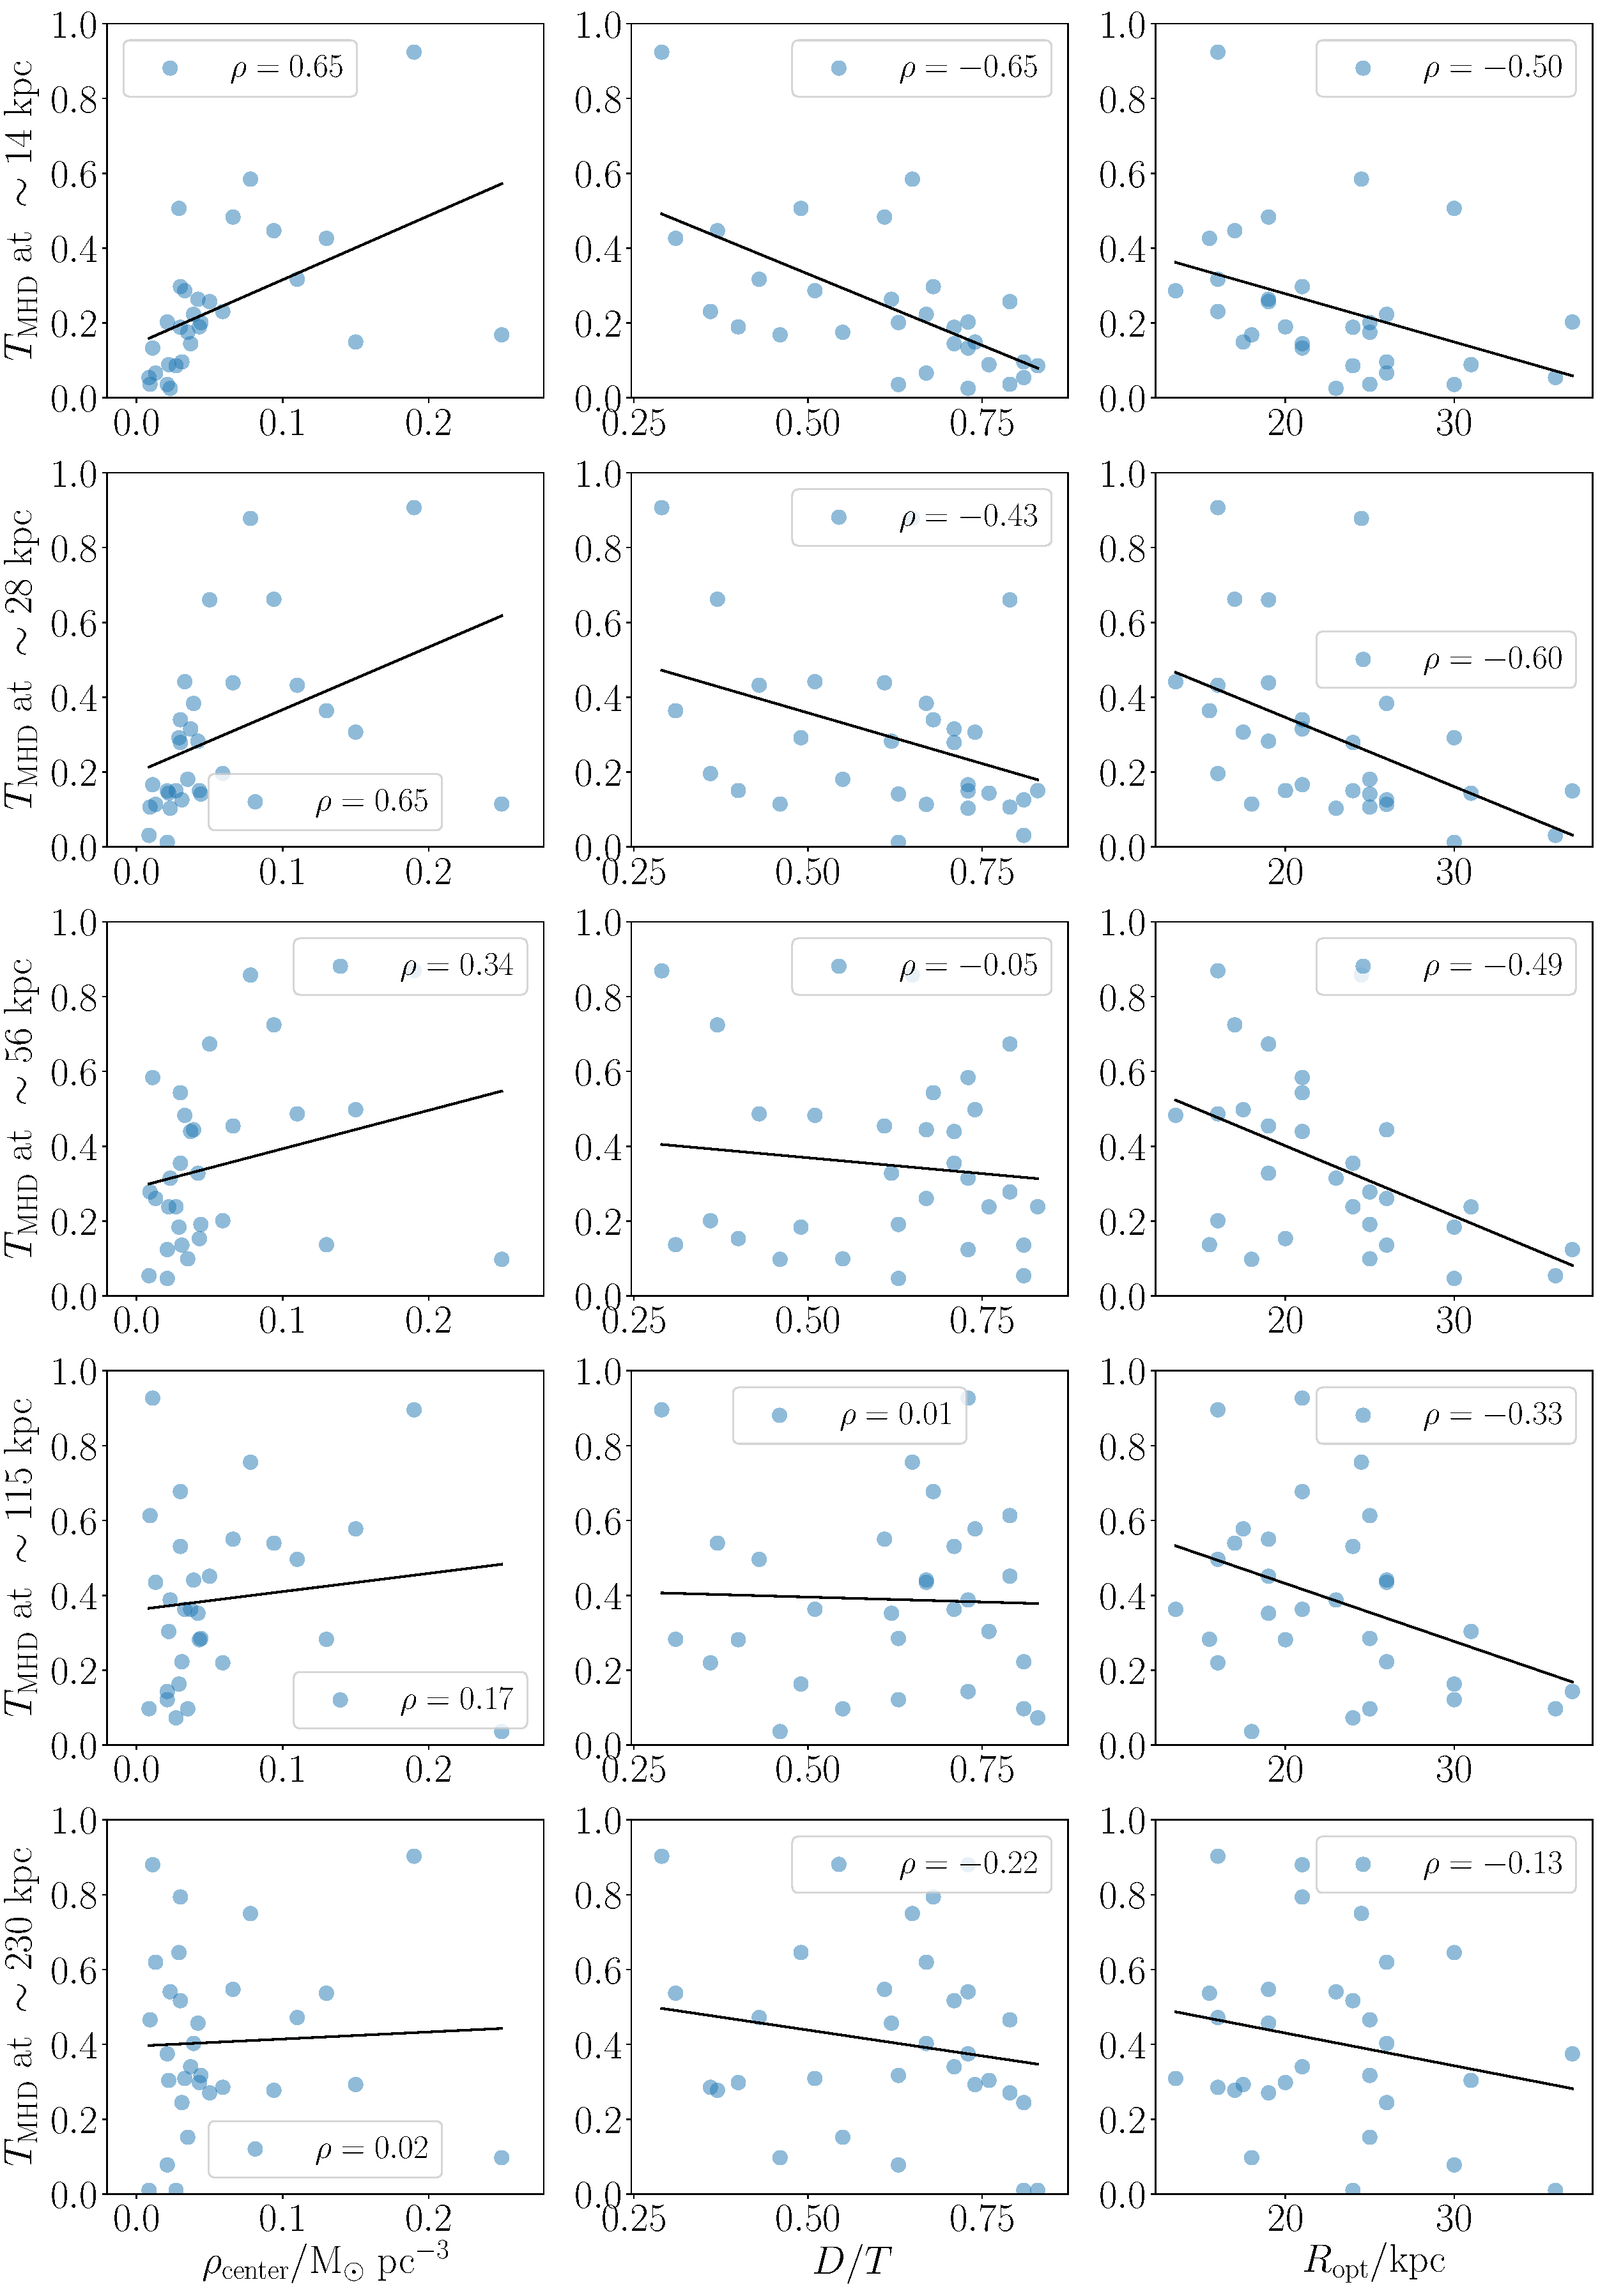
\includegraphics[width=0.8\textwidth]{correlation_T_MHD_disc.pdf}
\end{center}
\caption{Correlations between the halo triaxility at different radii
  and baryonic disc properties. 
  The label with the $\rho$ value corresponds to the Spearman's rank
  correlation coefficient.
  The line is the best linear minimum squares fit.
  The x-axis in the first column is the gas density at the center of
  the galaxy with in a sphere of radius  $1$ kpc \citep{Pakmor17};
  the second column shows the disc to total mass ratio and the last
  column includes the disc optical radius defined to be the radius at which the
  $B$-band surface brightness drops below 25 mag arcsec$^{-2}$ \citep{auriga}.
  The largest correlations are found for the two smaller radii and
  dilute as one approached $R_{200}$.
  Large and massive stellar discs with a low gas content are
  correlated with low dark matter triaxilities.}
\label{fig:disc_correlations}
\end{figure*}


\begin{figure*}
\begin{center}
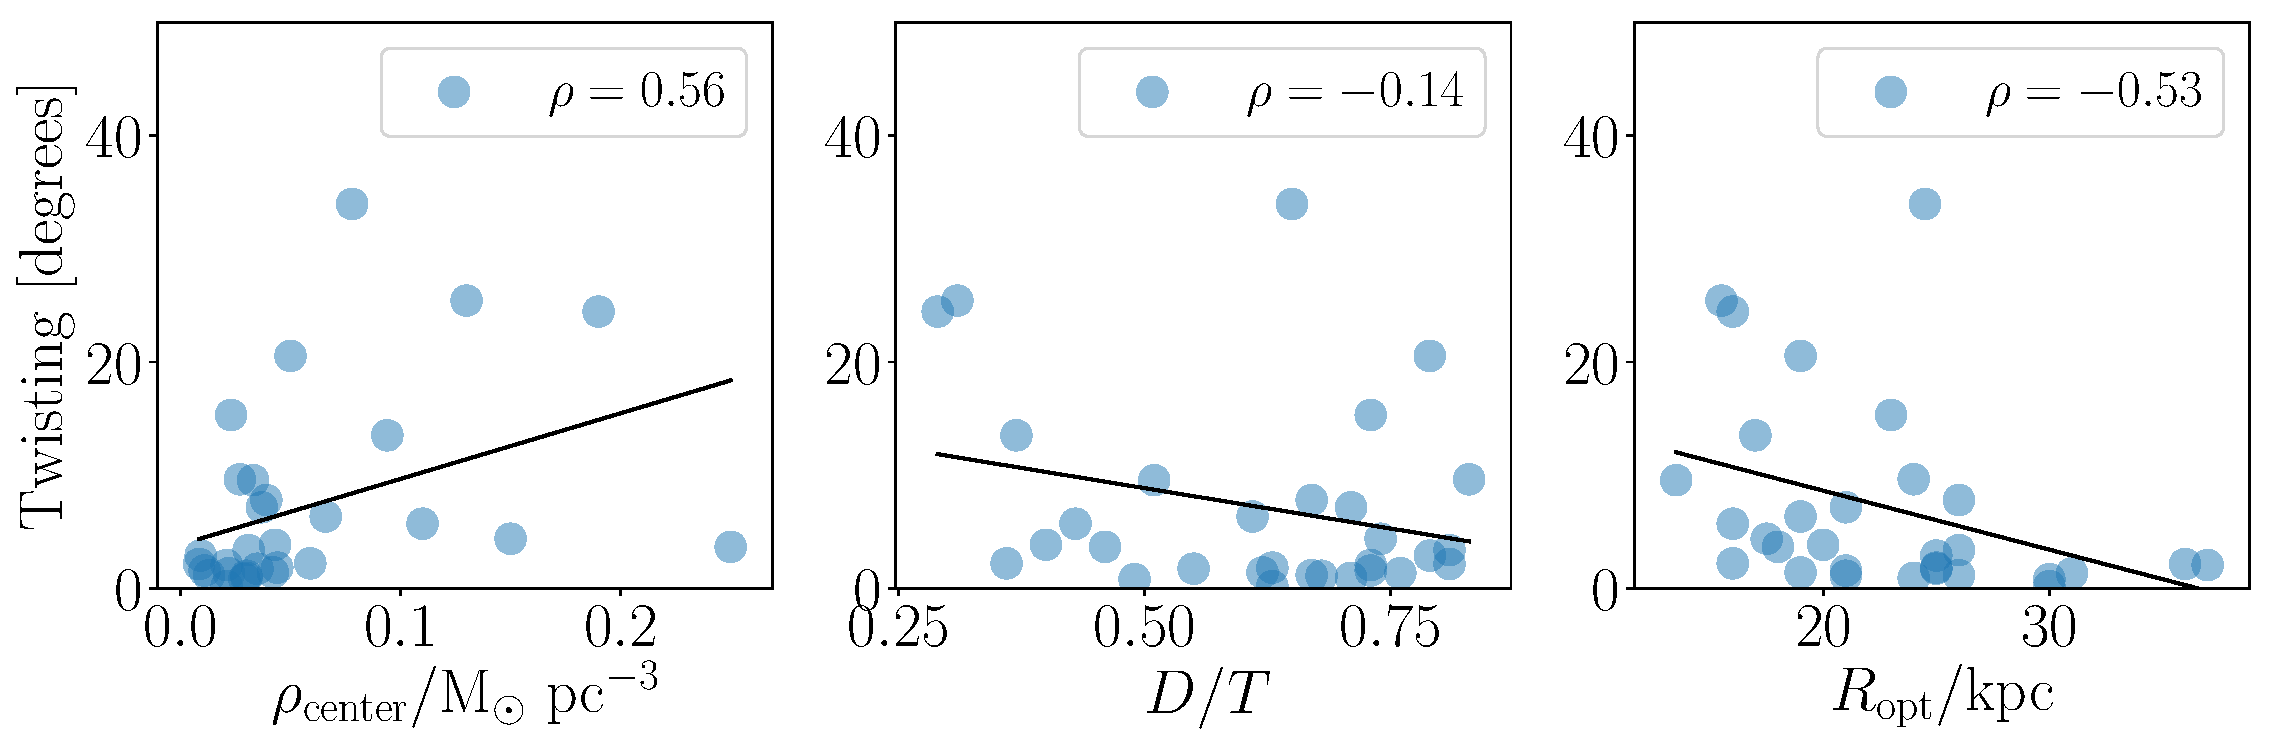
\includegraphics[width=0.9\textwidth]{correlations_angles_alignment_MHD.pdf}
\end{center}
\caption{Changse of angle alignment of the dark
  matter halo and stellar disc at two different radii ($R_{200}/16$
  and $0.25R_{200}$) as a function of the baryonic disc properties
  already explored in Figure \ref{fig:disc_correlations}.  
  Figure \ref{fig:cumulative_alignment} showed that maximum alignment
  occurs at $0.25R_{200}$ while in the inner regions ($R_{200}/16$)
  considerable missalignments occurr.
 at different radii
 and baryonic disc properties. 
 The label with the $\rho$ value corresponds to the Spearman’s rank correlation coefficient. }
\label{fig:alignment_correlations}
\end{figure*}



\begin{figure}
\begin{center}
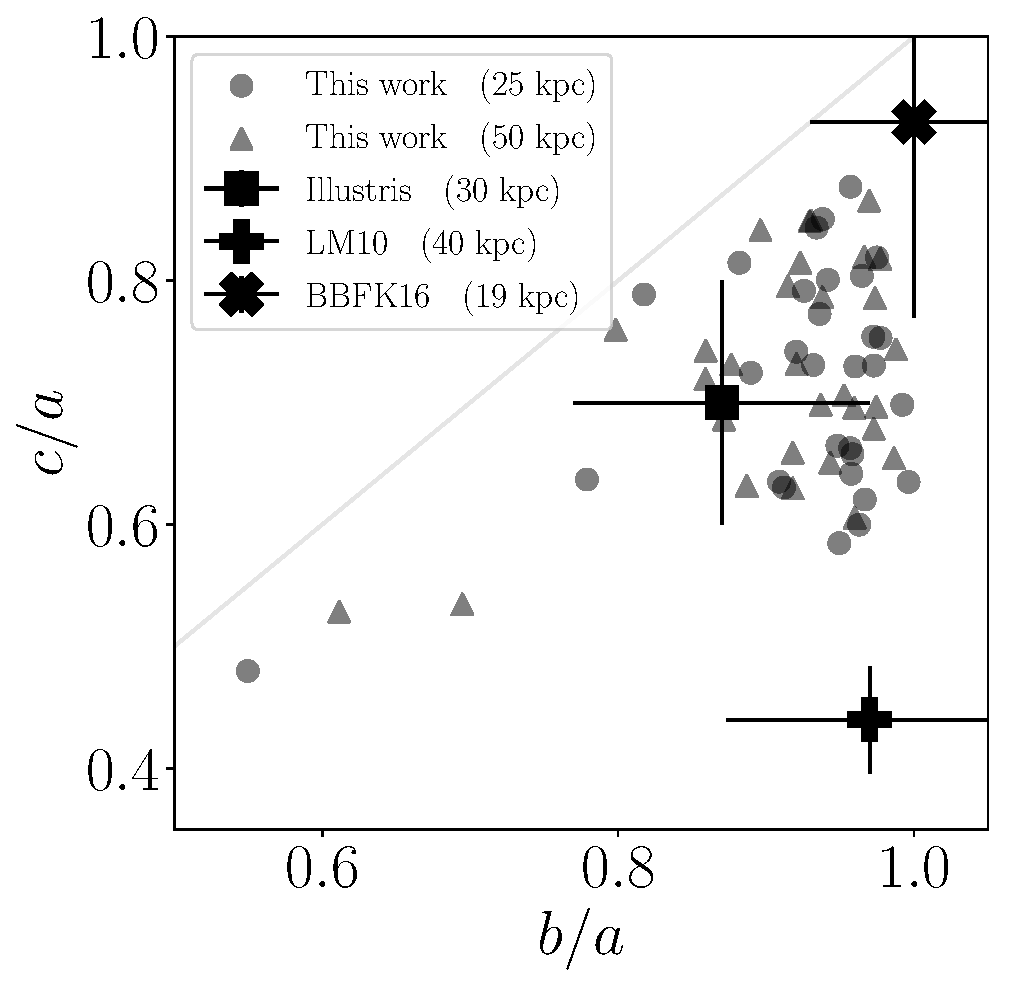
\includegraphics[width=0.45\textwidth]{triaxiality_observations.pdf}
\end{center}
\caption{Comparison of our results against 
observational constraints for the 
dark matter halo shape in the Milky Way by \citet{LM10} (LM10) and
\citet{Bovy16} (BBFK16).   
We find that  1/5 of the halos in the MHD  sample are consistent with
the constraints by \citet{Bovy16}.
In contrast, none of the halos in the MHD and DMO seems to be
consistent with the results by \citet{LM10}.}
\label{fig:observations}
\end{figure}


\section{Halo Shape Measurement}
\label{sec:method}

The DM halo shape at a fixed radius is an estimate of either
the isopotential or isodensity surfaces.  
Observational inference models usually estimate the 
isopotential contours which are probed by tracers (gas, stars), while
simulations work with the isodensity contours which can be directly
calculated from particle positions.  
Furthermore, the density contours in thin shells are very sensitive to
the presence of small satelites.  
For this reason we measure the shape by taking
volume-enclosed particles, rather than shell-enclosed.  
This method yields results in good agreement to the isodensity
contours for radii $\leq 140$ kpc as explored by
\citep{VeraCiro11}.  


In particular, we measure the shape using the reduced inertia tensor
\citep{Allgood06},  

\begin{equation}
I_{ij} = \sum_k \frac{x_k^{(i)}x_k^{(j)}}{d^2_k},
\label{eq:inertia}
\end{equation}

where the particle positions are measured from the minimum of the
gravitational potential in each halo and each is weighted by the k-th
particle distance $d_k^2=x_k^2+y_k^2+z_k^2$.

The diagonalization of this tensor yields the eigenvectors and
eigenvalues that represent an ellipsoidal dark matter halo.
The axis lenghts of this ellipsoid $a\geq b \geq c$ are the square
root of the ${\bf I}$ eigenvalues and the direction of the principal
axis are the corresponding eigenvectors 

We start the calculations taking into account particles within a
sphere of radius $R$ and then recharacterize the triaxial parameters
by taking into account particles within an ellipsoid of semi-axes
$r,r/q,r/s$ and re-scaled distance $d^2=x^2+(y/q)^2+(z/s)^2$, where $q
= b/a$ and $s=c/a$ are the previously calculated axial ratios. 
We repeat this process until the average deviation of semi-axes is
less than $10^{-6}$.  
After convergence we define a unique radius $R$ as the geometrical
mean of the axial lenghts $R=(abc)^{1/3}$.
We use this radial coordinate $R$ to parameterize the spatial changes
in halo shape we report in the following sections.

This is the same method used to estimate the halo shape in the DM-only
Aquarius simulations \citep{VeraCiro11}. 

Following the convergence criterion by \cite{VeraCiro11} we
restrict the sampling of the ellipsoidal parameters to radii  between
$\sim 2$kpc and $R_{200}$, where  $R_{200}$ correspond to the  radius
enclosing a sphere with 200 times the critical density of the Universe.
On average, over the 30 halos in the \texttt{Level4} sample
$R_{200}=230\pm 15$kpc. 


\section{Results}
\label{sec:results}

\subsection{Radial trends}

In the DMO sample we find that halos are rounder with increasing
radius.
The upper panels in Figure \ref{fig:slices} illustrate this effect.
The contours show a projected DM slice while the ellipsoid corresponds
to the full 3D shape determination. 
There we see a highly ellipsoidal halo shape at radii $\sim 3$kpc
that becomes less triaxial at $\sim 50$ kpc.

We summarize this trend in Figure \ref{fig:triaxiality_plane} by
plotting the results of all the 30 halos in the DMO sample.
The left panel shows every halo in the $c/a$-$b/a$ plane at
two different radii $R_{200}/8 (\sim 20$kpc$)$ and $R_{200}$. 
The outer part of the halo is systematically rounder than its inner
region. 
Nevertheless the halo shape can still be considerated to be prolate at
all radii. 
These plots confirm the results already reported in the
literature \citep{VeraCiro11}.

A different picture presents itself in the MHD sample.
There all halos become rounder at all radii than its DMO
counterpart.
The lower panel in Figure \ref{fig:slices} can be directly compared to
its MHD counterpart; there we observe how at large radii the halo
becomes almost spherical. 
The right panel in Figure \ref{fig:triaxiality_plane} shows the
results for the 30 halos in the MHD sample.
This time the bulk of the halos can be considered oblate and close to
spherical. 

In Figure \ref{fig:triaxial_cumulative} we summarize the results at
different radii using the cumulative distributions for the 
triaxility parameter $T$ defined as 

\begin{equation}
T=\frac{a^2-b^2}{a^2-c^2}.
\label{eq:triaxiality}
\end{equation}

The left panel of this Figure shows that in the DMO sample the
triaxility has a median larger than $0.5$ at all radii, furthermore
this median value increases as we move towards the inner part of the
halo.
The right panel shows the exact complementary picture in the MHD
sampe.
There the median triaxility is alwas smaller than $0.5$ and this
triaxility is smaller as we move closer to the galactic disc.


To quantify to what extend the global effect of decreasing
triaxility in MHD simulations compared to the DMO sample 
holds for individual halos. 
We compute $\Delta T\equiv T_{\rm MHD}-T_{\rm DMO}$ the difference between the
triaxility in the MHD and the DMO simulation for each individual halo. 
Figure \label{fig:delta_triaxial_cumulative} shows the cumulative
distribution at the same radii as in
Figure \label{fig:delta_triaxial_cumulative}. 
    

\subsection{Alignments with the stellar disc}


A common assumption in observational models of the MW DM halo is that
its minor axis is perfectly aligned with the stellar disc minor axis.
Although it is a reasonable assumption to guarantee the stability of
the galactic disc in simplified models of isolated galaxies, this
might not hold in an explicit cosmological context. 
To examine the degree of validity of this assumption we study in this
section the alignment between the eigenvectors of the inertia tensor of
stellar particles within $0.1R_{200}$ ($\sim 23\pm 2$ kpc) and the
eigenvectors of the dark matter halo shape.
All the measurements are done at $z=0$.

In Figure \ref{fig:cumulative_alignment} we summarize our main results
regarding these alignments with the halo shape measured at five
different radii.
The upper row shows the alignment of the halos in the DMO simulations
with the stellar disc in the MHD simulations.
The main objective of this measurement is to calibrate the radial
evolution of the DM halo shape. 
We find that the DM shape remains constant with radius.

The lower row in Figure \ref{fig:cumulative_alignment} shows the
alignments with the halo in the MHD simulations. 
This time the halo shape changes and twists at different radii.
However around the radius of $0.25R_{200}$ there is an alignment
almost perfect between the shapes of the stellar disc and the dark
matter halo. 
Above and below this radius there are halos with a lower degree of
alignment.
Across the three different alignments we measure we verify that the
strongest one is indeed the one between the two minor axis.

Statistically the strongest missalignment is found with the halo shape
at a radius of $R_{200}/16\sim (14\pm1)$ kpc. 
At this radius the mean angle and its standard deviation between the
two minor axis is $18 \pm 21$ degrees, with one extreme case
(\texttt{Au-4}) where the angle is close to $78$ degrees. 
In contrast at $0.25 R_{200}$ the angle between the two axis is
$2\pm 3$ degrees without any extreme outlier.





\section{Discussion}
\label{sec:discussion}

The first effect that we put in evidence in this paper is the effect
of baryons in producing rounder DM halos.

The strength of the change depends on the numerical resolution, the
method to resolve the hydrodynamics and the models describing star
formation and stellar feedback \citep{Debattista08, Bryan13, Butsky16,
  Chua19, Artale19}.  
The key concept unifying these results is that the baryon distribution
influences and correlates with the dark matter halo shape. 
Here we find that the broad tendency is that massive stellar discs
correlate with spherical dark matter distributions. 

In order to explore this idea in the Auriga simulations we quantify
the correlation between halo shape with baryonic disc properties. 
Looking into the measurements already reported by \cite{auriga} and
\cite{Pakmor17} we find three baryonic quantities that have the
strongest correlation with DM halo triaxiality: the central gas
density in a sphere of radius $1$kpc, the disc to total mass ratio and
the optical radius.

Figure \ref{fig:disc_correlations} shows the correlations of
these quantities with the triaxility at five diferent radii.
We use the Spearmen's rank correlation coefficient to quantify the
correlation strength.
We find that the strongest correlations are found with the halo shape
measured at radii smaller than $0.12R_{200}\sim 28$kpc, which 
is close to the upper limit of the disc optical radius among our
simulation sample. 
The trend is such that halos with large triaxiality correlate with
high gas density and stellar discs with low mass and small size.
In turn, massive and large stellar discs within a low density gas
environment correlate with low halo triaxiliaty. 

Our second results deals with the disc-halo shape alignment as a function of
radius. 
In concordance with previous results in DM only simulations we find
that the shells of halo shape are well aligned at different radii.
However, in the presences of baryons these shells twist as a function
of radius.
At a radius of $0.25R_{200}\approx 56$ kpc the alignment between the
stellar disc and the dark matter halo is almost perfect and degrades
at other radii. 
This twisting effect, the change of disc-halo alignment as
a function of radius, is robust across our sample of 30
halos at all radii.
However, its strenght is not the same for all galaxies and strongly
correlates with halo triaxiality measured at $0.12R_{200}$. 

\cite{Bailin05} studied the disc halo alignmnent as a function of
radius.
\cite{Gomez17} studied this in Auriga.
\cite{Debattista13} reported a similar twisting effect, but only at radii smaller
than the disc radius. 
At radii larger than the disc radius, they find, the dark matter
shells stop twisting. 
\cite{JingSuto02} also reported shell alignment twisting in their dark
matter only simulations as measured in the direction changes of large
and medium shape axis. 
They only had three high resolution MW-like halos (with
$\sim 10^{6}$ inside the virial radius) and could not make a
statistical statement about the impact of this effect.
However, they the twisting as an artifact resulting from high values of the
$c/b$ ratios that make the determination of the medium axis boisy.
Could then high triaxility values explain the twisting as a result of
erratic axis directions? 
If the triaxiality were the main culprit behind the twisting, the
correlation between the two quantities should be constant at every
radii.
In Figure \ref{fig:alignment_correlations} we already showed that this
correlation strongly depends on radius, we conclude that high
triaxiality values cannot be the full explanation.
Furthermore the twisting happens in such a way that it allows an
almost perfect alignment between the stellar disc at $0.1R{200}$ and
the halo shape measured at $0.25R_{200}$ 

We now use the results reported by \cite{LM10} and \cite{Bovy16}
to place our results in an observational context.
\cite{LM10} used observations of the Sagittarius tidal stream to
constrain the shape of the gravitational potential.
Their point of depart is that previous studies that assumed an
axisymetric galactic potential were not able to fit all the available
dynamic constraints for the Sagittarius stream, therefore making
necessary the use of a rigid triaxial potential with coaxial potential
ellipsoids for the dark matter component.  
Their results constrain the triaxility of this potential
component. 
They also translate ther results into a triaxiality of the density
contours (that could be compared against our results)
 to be $(c/a)=0.44$ and $(b/a)=0.97$ at a radius of $\sim 40$kpc. 
They do not report any uncertainties for these two values. 
Looking at their plots for the quality of fit criterion as a function
of dark halo axial scales (their Figure 5), we choose a conservative $10\%$
relative uncertainty.
One surprising element in their results is that  the major axis of the
halo shape is perpendicular to the stellar disc plane.  

The results by \cite{Bovy16} have the same general approach but use
instead the GD-1 \citep{2006ApJ...641L..37G} and Pal 5 \citep{2009AJ....137.3378O}
streams to constraint the shape of the dark matter component of the
galacic halo potential.
They use general models with many degrees of freedom for the galactic
potential in order to measure to what extent these two streams are sensitive
to the triaxiality of the dark matter halo component.
The DM component is written directly as a triaxial density profile
with coaxial ellipsoids and the corresponding potential is found by
numerical integration.
They find that the width of the Pal 5 stream constraints $b/a\approx
1$ and therefore fix it to be $b/a=1$ exactly.
Using that value they report their most stringent constrain of
$c/a=0.93\pm0.16$ at a radius of $\approx 19$kpc from the galactic
center. 

Our Figure \label{fig:observations} shows an explicit comparison in
the $c/a$-$b/a$ plane of our results in MHD simulations against the
results by LM10 and BBFK16.  
We find six MHD halos with $b/a<0.93$ and $c/a>0.77$ that could be
considered consistent with their shape constraints  by BBFK16, while
only one outlier DMO halo is consistent with those constraints.
In contrast, none of the simulated halos (MHD nor DMO) is consistent
with the LM10 results. 
The change of triaxility with radius in our simulations cannot account
for these two extremely different shape constraints at different
radii. 


The results by LM10 could then place the dark matter halo of our Milky
Way as an extreme outlier in the $\Lambda$ CDM model. 
This extreme prolateness also correlates with the extreme
triaxiality of the 11 classical satellites of the MW ($c/a\approx
0.2$, and $b/a\approx0.9$) with an spatial distribution 
also oriented perpendicular to the MW plane, another highly unusual
feature in the $\Lambda$ CDM model \citep{2018MNRAS.478.5533F}.


\section{Conclusions}
\label{sec:conclusions}

In this paper we measured the shape of 30 isolated Milky Way like 
dark matter haloes simulated in the Auriga project using the zoom-in
technique. 
The Auriga project simulated these halos with two different setups:
dark matter only (DMO) simulation and full magnetohydrodynamics (MHD)
including star formation and feedback.
We used the shape measurement algorithm by \cite{Allgood06} on the
dark matter halos of these two kinds of simulations to quantify the
halo shape as a function of radius and the degree of aligment between
the stellar disc and the halo.

We find that MHD halos are rounder than DMO halos at every radius.
MHD halos tend towards more oblate shapes ($T<1/3$), while DMO halos
tend towards more prolate shapes ($T>2/3$).  
The rounding effect is more noticeable as one moves closer to galactic
disc and strongly  correlates with baryonic properties of the disc
More precisely, the triaxility is smaller for large and massive
stellar discs with low gas densities at its core.

We also measured the shape alignment of the halo with the stellar
disc.
At a radius of $0.25R_{200}$ the alignment is almost perfect and
degrades at smaller and larger distances.
We found that in some halos the alignment betwen the stellar disc
and dark matter halo changes noticeably with the radius.
This alignment evolution implies a radial twisting between the ellipsoids
describing the halo shape. 
We quantify this twist with the standard deviation of the angle
between the two minor axis at radii below $\leq 0.5R_{200}$ and find
that it strongly correlates with the disc size and the core gas
mass density, there is only a weak correlation with the disc to
total mass ratio in the disc.

We compared our results against two observational constraints for the
dark matter halo shape of the Milky Way. 
The constraints are at two different radii and come from different
observatinal tracers. 
We find that $20\%$ halos in the MHD simulations are consistent with
the constraints by \cite{Bovy16} at $\approx 19$kpc, while none of the
halos, either in MHD or DMO, has some overlap with the shape
constraints by \cite{LM10} at $\approx 40$kpc. 

From the results presented in this work we advance the idea that the
twisting shells in the density is a feature that deserves to be
explored in the process of constraining shape parameters from tidal
stream data. 
The inclusion of a parameterization describing this degree of
twisting might relax the conflict between the observational
constraints and the numerical results. 

From the purely numerical point of view a better understading of the
disc-halo alignment details will certainly require to study how the
halo and the disc co-evolved as a function of time.
Calibrating the effect of the cosmic web (both dark matter and gaseous)
\citep{2014MNRAS.443.1090F,2017MNRAS.469..594B,2019MNRAS.487.1607G}
could also be required to gain a full picture of this behaviour.  


\section*{Acknowledgements}
This project has received funding from the European Union's Horizon
2020 Research and Innovation Programme under the Marie
Sk\l{}odowska-Curie grant agreement No 734374. 

 \bibliographystyle{mnras}
 \bibliography{references}

\end{document}


